\documentclass[aps,%
12pt,%
final,%
oneside,
onecolumn,%
musixtex, %
superscriptaddress,%
centertags]{article} %%
\topmargin=-40pt
\textheight=650pt
\usepackage[english,russian]{babel}
\usepackage[utf8]{inputenc}
%всякие настройки по желанию%
\usepackage[colorlinks=true,linkcolor=blue,unicode=true]{hyperref}
\usepackage{euscript}
\usepackage{supertabular}
\usepackage[pdftex]{graphicx}
\usepackage{amsthm,amssymb, amsmath}
\usepackage{textcomp}
\usepackage[noend]{algorithmic}
\usepackage[ruled]{algorithm}
\usepackage{geometry}
\usepackage{setspace}
\geometry{verbose,a4paper,tmargin=2cm,bmargin=2cm,lmargin=3cm,rmargin=1cm}
\onehalfspacing
\selectlanguage{russian}

\begin{document}

\begin{titlepage}
\begin{center}
% Upper part of the page
\textbf{\Large САНКТ-ПЕТЕРБУРГСКИЙ \\ ГОСУДАРСТВЕННЫЙ УНИВЕРСИТЕТ} \\[1.0cm]
\textbf{\large Математико-Механический факультет} \\[0.2cm]
\textbf{\large Кафедра информационно аналитических систем}\\[3.5cm]

% Title
\textbf{\LARGE Суммаризация групп в социальных сетях}\\[1.0cm]
\textbf{\Large Дипломная работа студента 646 группы} \\[0.2cm]
\textbf{\Large Чурикова Никиты Сергеевича} \\[3.5cm]

%supervisor
\begin{flushright} \large
\emph{Научный руководитель:} \\
к.ф. - м.н., доцент \textsc{Графеева Н. Г.}
\end{flushright}
 \begin{flushright} \large
\emph{Рецензент:} \\
% TODO: Убрать биологию
Директор департамента управления информационными потоками \textsc{Яковлев П. А.}
\end{flushright}
\begin{flushright} \large
\emph{Заведующий кафедрой:} \\
к.ф. - м.н., доцент \textsc{Михайлова Е. Г.}
\end{flushright}
\vfill

% Bottom of the page
{\large {Санкт-Петербург}} \par
{\large {2019 г.}}
\end{center}
\end{titlepage}

\begin{titlepage}
\begin{center}
% Upper part of the page
\textbf{\Large SAINT PETERSBURG STATE UNIVERSITY} \\[1.0cm]
\textbf{\large Mathematics and mechanics department} \\[0.2cm]
\textbf{\large Sub-Department of Analytical Information System}\\[3.5cm]

% Title
\textbf{\LARGE News resources summarization in social networks}\\[1.0cm]
\textbf{\Large Final thesis of student of 646 group} \\[0.2cm]
\textbf{\Large Churikov Nikita Sergeevich} \\[3.5cm]

%supervisor
\begin{flushright} \large
\emph{Scientific Supervisor:} \\
Assistant Professor \textsc{Grafeeva N. G.}
\end{flushright}
 \begin{flushright} \large
\emph{Reviewer:} \\
% TODO: Убрать биологию
Director of information flow department \textsc{Yakovlev P. A.}
\end{flushright}
\begin{flushright} \large
\emph{Sub department director:} \\
Assistant Professor \textsc{Michailova E. G.}
\end{flushright}
\vfill

% Bottom of the page
{\large {Saint Petersburg}} \par
{\large {2019 г.}}
\end{center}
\end{titlepage}

% Table of contents
\tableofcontents

\section{Аннотация}
Одной из задач обработки естественного языка является задача суммаризации текста.
Ее целью является уменьшение размера исходного текста без потери ключевой информации.
В данной работе мы решаем схожую проблему, но для информационных ресурсов в социальных сетях.
В частности, мы рассматриваем задачи генерации заголовков и выделения ключевых слов,
поскольку тексты бывают разного объема и потому их можно сжимать разными способами.
В тексте мы приводим численное обоснование выбранных методов и описываем интерфейс разработка.

\section{Введение}
В современном мире создается все больше и больше информации, которую мы можем потреблять.
Новости, статьи, юмор постоянно меняются и создаются людьми. При таком потоке информации
появляется потребность в инструментах, способных давать как можно больше информации
с минимальными потерями.

При чтении новостей люди, как правило, не идут дальше новостных заголовков \cite{jaysondemers2016},
для популярных технических статей создают краткие описания описывающие их достижения
и основные моменты \cite{tldr_arxiv2019, articleessence2019}, а визуальный контент нередко подчиняется единому шаблону.

В данной работе мы показываем, как используя современные достижения в области анализа
данных можно извлекать полезную информацию из новостных ресурсов в социальной сети вконтакте \cite{vk2019},
и приводим обоснование выбора решений, основываясь на соответствующих метриках.

\subsection{Постановка задачи и описание требований}
Мы поставили перед собой задачу создать систему, которой бы можно было передавать ссылку на новостной ресурс в социальной сети вконтакте, а на выходе получать его краткое описание. В рамках работы мы ограничились новостными ресурсами с высоким содержанием текста.

На Рис. \ref{app_story} мы показываем как работает наше решение "с высоты птичьего полета". Процесс имеет следующий вид, мы получаем ссылку на группу ВК, затем через API вконтакте получаем информацию о группе и оцениваем количество текста в ней. если содержание текста низкое, то мы говорим, что это ресурс с доминирующим медиа-контентом, если в группе мало предложений, но достаточно слов, то решается задача выделения ключевых слов, если в группе высокое содержание предложений, то мы решаем задачу генерации заголовков.

Таким образом, с алгоритмической точки зрения, задача суммаризации новостного ресурса была рассмотрена нами как две подзадачи:
\begin{enumerate}
  \item Извлечение ключевых слов, присущих данному источнику информации;
  \item Сжатие новостей, используя автоматическое создание заголовков.
\end{enumerate}

Через извлечение данной информации мы хотим добиться эффекта "чтения по диагонали".

Для оценки качества наших алгоритмов, мы воспользовались открытыми датасетами для генерации заголовков и извлечению ключевых слов.

\begin{figure}[ht]
\begin{center}

\scalebox{0.6}{
   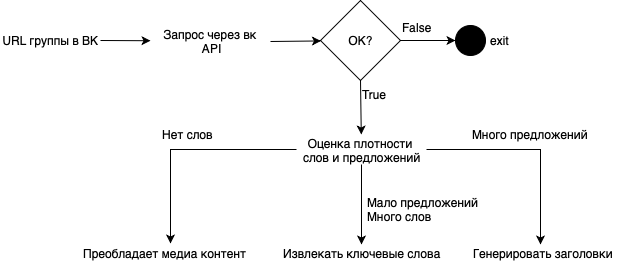
\includegraphics{images/app_story.png}
}

\caption{
\label{app_story} Принцип работы системы.
        }
\end {center}
\end {figure}

Рассмотрим теперь то, насколько актуальна данная проблема
и какое место занимает предлагаемое решение среди существующих систем анализа
групп в социальных сетях.

На рынке уже существует большое множество сервисов дающих возможность проанализировать группу
на предмет возможного размещения рекламного поста \cite{smmpub2019}. Однако несмотря на
такое разнообразие сервисов, их функционал слабо отличается друг от друга. Как правило, предоставляется
возможность следить за аудиторией (ее полом, численностью, возрастом), частотой выпускаемого материала,
частотой выпуска материала и его типом. Однако никто из игроков не производит анализа содержания групп,
что кажется упущением возможности выделиться на рынке.

Наличие анализа содержания группы могло бы повысить скорость создания рекламы за счет уменьшения времени, необходимого для того, чтобы вникнуть в идею группы.

Причинами того, что создатели подобных сервисов не спешат с созданием таких услуг мы видим следующее:
\begin{itemize}
  \item Необходимо нанимать новых сотрудников, что влечет дополнительные расходы;
  \item Спрос на подобный функционал может быть низок из-за того, что в случае успеха подобного функционала, может снизиться спрос на специалистов в области SMM.
  \item Поскольку спрос низкий, то данное предложение не предлагается.
\end{itemize}

Имея ввиду причины отсутствия подобного функционала, мы считаем, что есть смысл создать его в виде
черной коробки, которую можно будет подключать к уже существующим сервисам. В этой черной коробке
использовать алгоритмы, которые показали отличные результаты на академических датасетах и рекомендовать их как базовые, однако оставить выбор за разработчиками при выборе алгоритмов.

Таким образом стоят следующие задачи:

\begin{itemize}
  \item Проанализировать существующие алгоритмы выделения ключевой информации из текстов;
  \item Предоставить возможность воспользоваться этими решениями как черным ящиком, создав интерфейсы для разработчиков:
  \begin{itemize}
    \item Библиотеку на python
    \item REST API, чтобы была возможность использовать из других языков программирования
  \end{itemize}
\end{itemize}

\subsection{Обзор литературы}
Задача сжатия текста с малой потерей смысла и сохранением возможности его прочтения
имеет название задачи \textit{суммаризации}. При этом, есть два концептуальных подхода к решению:
экстрактивный, когда для создания краткого содержания извлекаются целые куски текста вплоть до предложений,
и абстрактивная, где в кратком содержании могут быть слова, которых не было в исходном тексте.

В частности, при исследовании абстрактивной генерации заголовков, мы отталкивались от статьи Вконтакте, посвященной данной проблеме \cite{gavrilov2018self}. Ими предлагается применять нейронные сети с архитектурой Transformer и предобработкой Byte pair encoding (BPE) \cite{DBLP:journals/corr/SennrichHB15}. Однако в задаче абстрактивной генерации заголовков существуют дебаты на тему того, что использовать в качестве входа модели. Поскольку долгое время SOTA были модели с архитектурой encoder decoder, то было невозможно использовать длинные входные последовательности. Потому авторы статьи \cite{Putra2018IncorporatingTS} исследуют различные подходы по предварительному извлечению "Topic sentence", которое нейронная сеть должна дальше обработать. Это предложение, как говорят авторы, в идеальном случае, должна отвечать на 5W1H. Но достаточно ответов на "что, кто, когда".

Для экстрактивной суммаризации чаще всего используют алгоритм TextRank \cite{TextrankOriginal}.
% TODO: Add more desctiption
% https://docplayer.ru/26752739-Vydelenie-klyuchevyh-slov-v-russkoyazychnyh-tekstah.html
% http://www.dialog-21.ru/media/3995/sandrikova.pdf
% YAKE
% https://repositorio.inesctec.pt/bitstream/123456789/7623/1/P-00N-NF5.pdf
% Браславский


% \subsection{Полученные результаты}
% Что является результатом работы (будет веб сервис, куда можно закинуть ссылку на группу),
% как оценивали качество (продолжить результаты работы алгоритмов толокерам), а также
% оценка качества по автоматизированным метрикам, и как они коррелируют с оценками людей.
% Сравниться с бэйзлайном.

\section{Описание системы}

\section{Алгоритмы, использованные в работе}
Нами были использованы как классические подходы, так и новые, основанные на нейронных сетях.
В следующих секциях мы опишем их основные принципы, а также приведем ссылки на их реализации.

\subsection{Суммаризация текста}
Для суммаризации текста мы воспользовались алгоритмом экстрактивной суммаризации
основанном на TextRank \cite{DBLP:journals/corr/BarriosLAW16, rehurek_lrec, TextrankOriginal},
и моделью трансформера \cite{DBLP:journals/corr/VaswaniSPUJGKP17}, обученной на
датасете РИА новостей \cite{gavrilov2018self}.
Для предобработки данных модели трансформера мы использовали byte
pair encoding \cite{DBLP:journals/corr/SennrichHB15}.
Помимо этого мы извлекали первое предложение из новости.
Для TextRank и извлечения первого предложения не требуется обучающая выборка, что
делает их очень удобными в использовании. При этом, исследования показывают, что
в задаче генерации заголовков, первое предложение в новости --
это очень сильный бэйзлаин \cite{gavrilov2018self},
который трудно побить как экстрактивной, так и абстрактивной суммаризацией.

\subsubsection{Baseline}

В качестве бэйзлаина в задаче генерации заголовков используется первое предложение новости. Именно им мы и воспользовались и отталкивались от него.


\subsubsection{TextRank}

TextRank является является адаптацией идеи алгоритма PageRank \cite{Page98thepagerank} с задачи рекомендации страниц в интернете на задачу рекомендации лучшего предложения или набора слов в тексте. Сам алгоритм состоит в том, что мы текст превращаем в граф, где узлы -- это предложения, а для каждого ребра подсчитывается вес, где вес определяется по количеству совпавших слов в двух предложениях.

Таким образом, получается, что можно выбрать предложение с самыми тяжелыми ребрами в качестве предложения, которое описывало бы исходный текст.

\begin{figure}[ht]
\begin{center}

\scalebox{0.4}{
   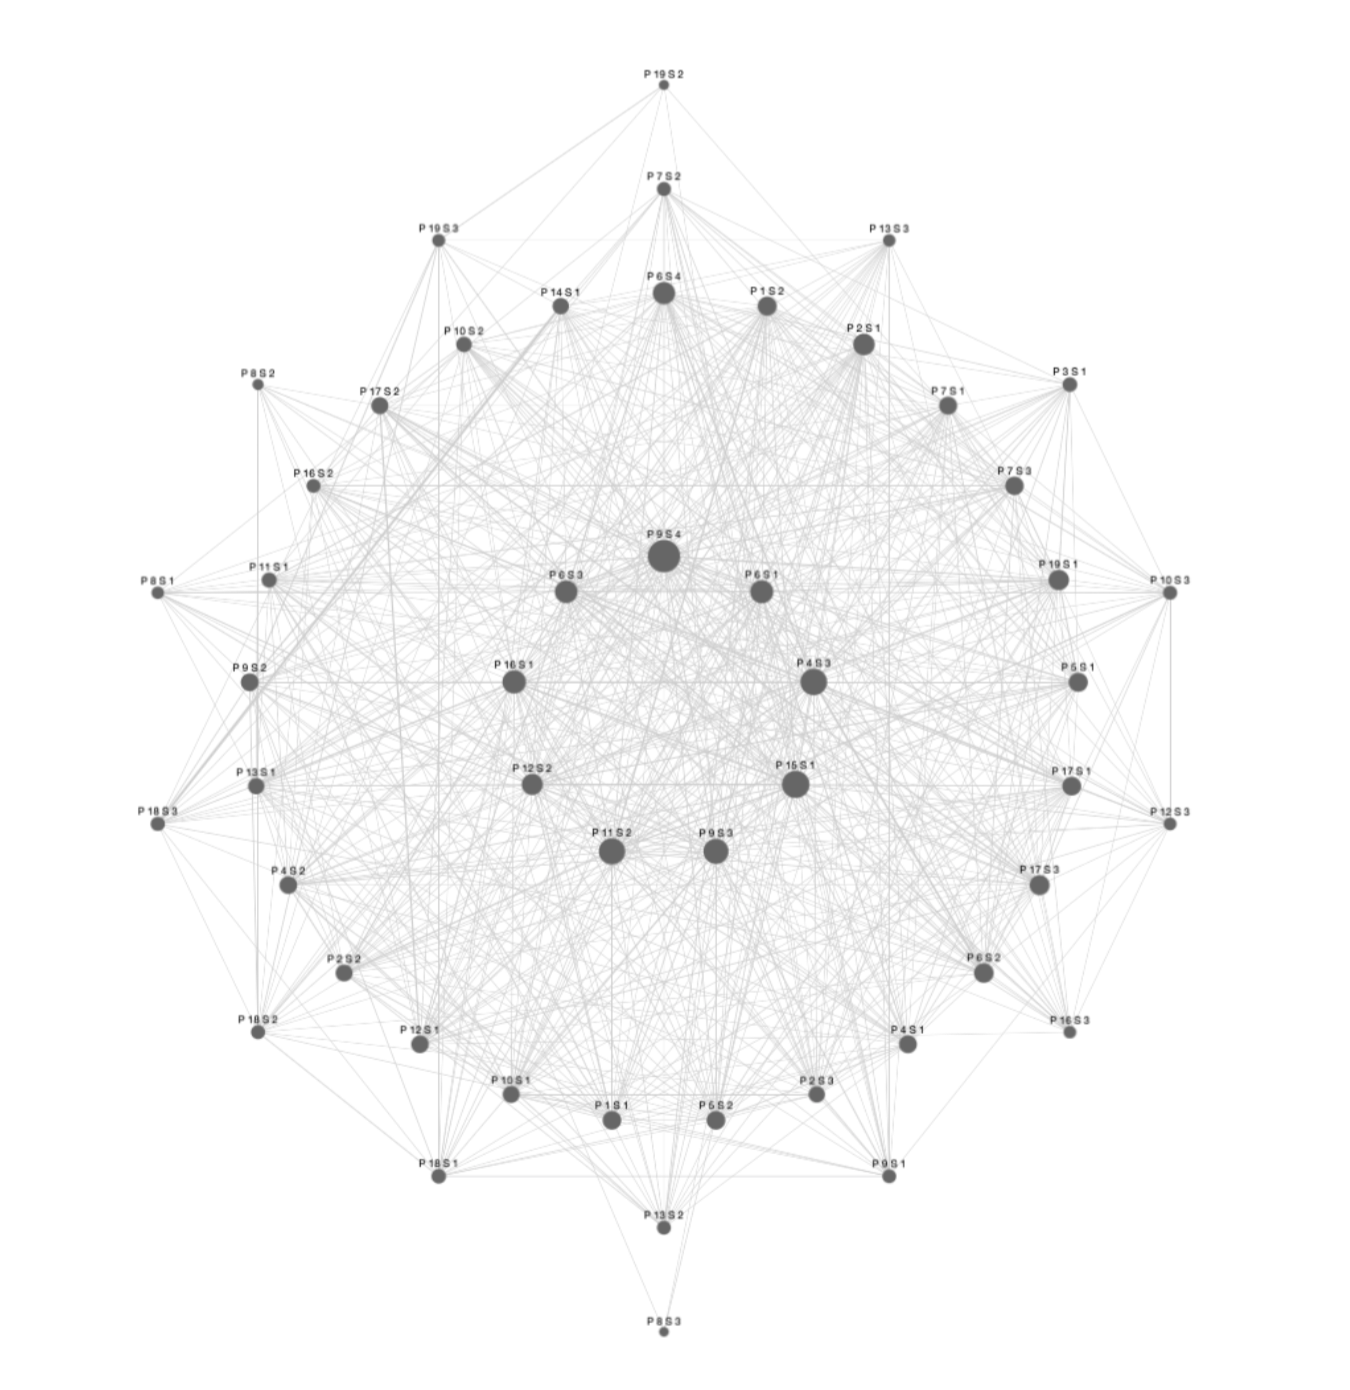
\includegraphics{images/text_rank_example_graph.png}
}

\caption{
\label{text_rank_example_graph}
        Пример результирующего графа textrank.}
\end {center}
\end {figure}

\subsubsection{Byte pair encoding}

Мы используем byte pair encoding (BPE), технику, предложенную Сеннрич для задачи машинного перевода в \cite{DBLP:journals/corr/SennrichHB15}. BPE -- это метод сжатия данных, в котором часто встречающиеся пары байтов заменяются дополнительными символами алфавита. В случае текстов, как в области машинного перевода, наиболее часто встречающиеся слова сохраняются в словаре, а менее часто встречающиеся слова заменяются последовательностью (обычно двумя) токенами. Например, для морфологически богатых языков окончания слов могут быть отделены, поскольку каждая форма слова определенно реже, чем ее основа. Кодирование BPE позволяет нам представлять все слова, включая те, что не встречаются по время обучения, с фиксированным словарным запасом.

% \subsubsection{Beam search}


\subsubsection{Universal transformer network}
В то время как рекуррентные нейронные сети могут быть легко использованы для определения модели Encoder-Decoder, тренировка таких моделей очень дорого с точки зрения вычислений. Другой недостаток состоит в том, что они используют только локальную информацию, опуская последовательность скрытых состояний H = {h1, ..., hN}. То есть любые два вектора из скрытого состояния hi и hj связаны с вычислениями j - i RNN, что затрудняет улавливание всех зависимостей в них из-за ограниченной емкости. Чтобы обучить богатую модель, которая изучила бы сложную текстовую структуру, мы должны определить модель, которая опирается на нелокальные зависимости в данных.
В этой работе мы принимаем архитектуру модели Universal Transformer \cite{}, которая является модифицированной версией Transformer \cite{}. Этот подход имеет несколько преимуществ по сравнению с RNN. Прежде всего, его можно тренировать параллельно. Кроме того, все входные векторы связаны друг с другом через механизм Attention. Это подразумевает, что архитектура Transformer учитывает нелокальные зависимости между токенами независимо от расстояния между ними, и, таким образом, она может выучить более сложное представление текста в статье, что оказывается необходимым для эффективного решения задачи суммаризации.

\subsection{Выделение ключевых слов}

Статья Boudin, Florian \cite{boudin:2016:COLINGDEMO} рассматривает наиболее сильные подходы к выделению ключевых слов.
И основная суть их статьи в том, что они предлагают реализации основных алгоритмов выделения ключевых слов, однако проблема,
с которой мы столкнулись состоит в том, что в ядре их библиотеки заложена библиотека spacy \cite{honnibal-johnson:2015:EMNLP}, которая не работает с русским языком
% Конкретно, они показывают для каких задач доходят какие алгоритмы. Основная таблица этой статьи приведена на таблице \ref{keywords_extraction_report},
% и она говорит о том, какие алгоритмы показывают лучшие результаты на каких задачах.

Таким образом, для данной работы мы реализовали TopicRank, TfIdf и YAKE поскольку эти алгоритмы являются лучшими алгоритмами для выделения ключевых слов. Мы выложили эти реализации в качестве библиотеки на python \footnote{https://github.com/kuparez/keyverbum}, реализовав интерфейсы библиотеки Scikit-Learn \cite{scikit-learn, sklearn_api}.

% \begin{table}[ht]
%   \begin{center}
%     \begin{tabular}{|l|l|l|l|l|}
%       \hline
%       \textbf{Dataset} & \textbf{Approach and System} & \textbf{P} & \textbf{R} & \textbf{F} \\ \hline
%       Абстракты & TopicRank & 35.0 & 66.0 & 45.7 \\ \hline
%       Блоги & CommunityCluster & 35.1 & 61.5 & 44.7 \\ \hline
%       Новости & \begin{tabular}[c]{@{}l@{}} TextRank \end{tabular} & 28.8 & 35.4 & 31.7 \\ \hline
%       Научные статьи & \begin{tabular}[c]{@{}l@{}}Statistical, semantic, \\ and distributional features\end{tabular} & 27.2 & 27.8 & 27.5 \\ \hline
%     \end{tabular}
%     \caption{
%       \label{keywords_extraction_report} Sate of the art результаты извлечения ключевых слов на классических датасетах. P -- точность, R -- полнота, F -- среднее гармоническое точности и полноты.
%     }
%   \end{center}
% \end{table}

В секциях ниже мы опишем детали наших реализаций данных алгоритмов.

\subsubsection{TopicRank}
TopicRank - это метод обучения без учителя, целью которого является извлечение ключевых фраз из наиболее важных тем документа. Темы определяются как кластеры похожих ключевых фраз-кандидатов. Извлечение ключевых фраз из документа состоит из следующих шагов, показанных на рисунке \ref{topicrank}. Во-первых, документ предварительно обрабатывается (сегментация предложений, разметка слов и тегирование частей речи), а кандидаты в ключевые фразы группируются по темам. Затем темы ранжируются в соответствии с их важностью в документе, и ключевые фразы извлекаются путем выбора одного кандидата ключевой фразы для каждой из наиболее важных тем.

\begin{figure}[ht]
\begin{center}

\scalebox{0.4}{
   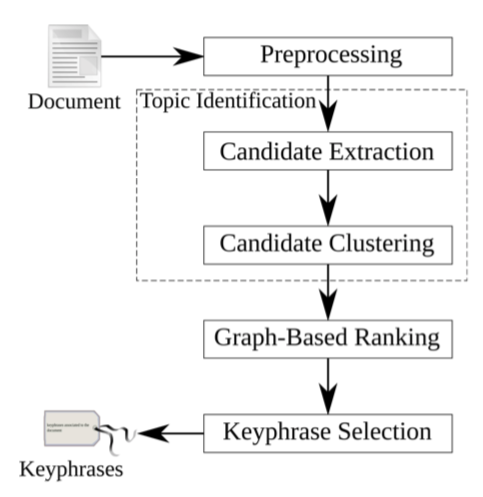
\includegraphics{images/how_topicrank_works.png}
}

\caption{
\label{topicrank}
        Принцип работы TopicRank.}
\end {center}
\end {figure}

% \subsection{Суммаризация изображений}
% Для суммаризации изображений мы реализовали алгоритм,
% описанный в статье \cite{DBLP:conf/icsipa/SharmaKASK15}.
% Основная идея состоит в том, что из изображений извлекаются
% признаки, инвариантные к поворотам \cite{Lowe:2004:DIF:993451.996342},
% эти признаки кластеризуют
% используя k-means \cite{Arthur:2007:KAC:1283383.1283494} и индексы кластеров
% используют как признаки для латентного размещения
% Дирихле \cite{Blei:2003:LDA:944919.944937, rehurek_lrec}.
%
% Помимо этого, мы попробовали
% на нашей задаче обучению метрике между изображениями
% \cite{DBLP:journals/corr/abs-1803-11095, DBLP:journals/corr/abs-1810-06951}.

\subsubsection{YAKE}


\subsection{Оценки качества}
Для оценки качества текстовых моделей мы использовали метрику ROUGE-L F1 \cite{Lin:2004},
при этом мы считали ее на датасете РИА новостей \cite{gavrilov2018self}. Помимо этого,
на основе этого датасета проводилось соревнование по генерации заголовков, где автором было
получено 3 место, а описание результатов соревнования было подано в качестве статьи на конференцию
"Диалог".

% Помимо этого, как для текстовых данных, так и для изображений, мы  использовали
% Яндекс.Толоку \cite{yandex_toloka_2019}, чтобы привлечь людей к оценке качества наших результатов.


\section{Анализ использованных данных}
% Рассказать про датасет Риа новостей и данные из ВК.

В работе были использованы несколько датасетов с целью выбора алгоритмов под соответствующие задачи.
В частности, мы воспользовались датасетом оценки качества выделения ключевых слов \cite{mannefedov2019}, недавно
опубликованным датасетом Риа новостей \cite{gavrilov2018self}, а также в нашей работе мы используем
данные из 25 групп вконтакте с разным целевым материалом: от медиа контента до полноценных длинных
текстов.

\subsection{Данные выделения ключевых слов}

\begin{table}[ht]
  \begin{center}
    \begin{tabular}{|l|l|l|l|}
      \hline
      \textbf{Датасет} & \textbf{Тип} & \textbf{\begin{tabular}[c]{@{}l@{}}Количество \\ документов\end{tabular}} & \textbf{\begin{tabular}[c]{@{}l@{}}Среднее \\ количество \\ токенов\end{tabular}} \\ \hline
      Киберленика & Абстракты & 4072 & 5.27 \\ \hline
      Habr & Блоги & 3990 & 5.03 \\ \hline
      Независимая газета & Новости & 1987 & 6.11 \\ \hline
      Россия сегодня & Новости & 7217 & 10.07 \\ \hline
    \end{tabular}
  \end{center}
\end{table}

Для анализа качества использованных алгоритмов для выделения ключевых слов
мы воспользовались датасетом с разнообразными статьями на русском языке \cite{mannefedov2019}.
В наборе присутствуют научные статьи из "журнала киберленика" \cite{cyberlenica},
технического блога "хабрахабр" \cite{habr} и новостных ресурсов "Независимая газета" \cite{independentjournal} и "Россия сегодня" \cite{rt}.

% Таким образом, мы приводим русскоязычные аналоги всем англоязычным ресурсам из таблицы \ref{keywords_extraction_report}.

\subsection{Данные для генерации заголовков}

Для обучения и выбора алгоритмов генерации заголовков, мы воспользовались недавно опубликованным
датасетом Риа новостей. Этот датасет содержит новости с января 2010 по декабрь 2014.
В нем имеется 1003869 новостных статей со средним размером заголовка 9.5 слов и
средней длинной текста 315.6 слов.

Эти датасет предоставлен в виде необработанных фрагментов оригинальных html-страниц.
Это означает, что в данных присутствовали различные HTML-теги и объекты.
В итоге имеется необработанная новость и соответствующий заголовок.

\begin{verbatim}

<p> <strong> <\strong> <\p> \n <p> <strong> Moscow,
Dec 1 &nbsp; &mdash; RIA news. <\strong> a fire in &nbsp;
one of the &nbsp; workshops in &nbsp;...<\p>
\end{verbatim}

В результате первым делом мы попытались очистить данные от ненужной информации. И так, мы создали препроцессор, который удаляет все html-теги и сущности.

Кроме того, мы обнаружили, что иногда в данных отсутствует текст, поскольку исходные новости представлены в виде изображений (например, снимок экрана Twitter), а новости чисто польские. Это все выбросы, с которых мы очистили данные.


\section{Эксперименты}
В данной секции мы приводим технические детали, параметры моделей и оценки качества созданных моделей на датасетах описанных выше.

\subsection{Генерация заголовка}
На практике обычно используется метрика ROUGE \cite{Lin: 2004} при оценке качества алгоритмов суммаризации. Конкретно используются так называемые ROUGE 1,2, L - точность, полнота и F1. Имена в ROUGE X - Y обозначают следующее: X - количество n-грамм, используемых для вычисления метрики Y. В случае n-грамм размера L рассматривается самая длинная общая подпоследовательность из предсказанной последовательности найденая в исходной последовательности. Метрики Y - классическая точность, полнота и их среднее гармоническое.

В случае алгоритма Textrank \cite{DBLP:journals/corr/BarriosLAW16}, алгоритма экстрактивной суммаризации, мы воспользовались реализацией из библиотеки gensim \cite{rehurek_lrec}. В случае этого алгоритма, выделяется не одно предложение, а подмножество текста определенного размера, потому мы установли параметр отвечающий за размер возвращаемого текста равным 20\% от исходного.

Мы взяли state of the art реализацию алгоритма Universal Transformer из Open NMT \cite{2017opennmt} и обучили этот алгоритм на данных Риа новостей. Мы использовали 4 слоя кодировщика и декодеривщика, 8 heads of attention, вероятность дропаута была выставлена равной 0.3. Для оптимизации был использован алгоритм Adam с изменяющейся скоростью обучения, по правилу из оригинальной статьи о трансформере.

В качестве входа модели мы использовали первые 2000 BPE токенов.

Что касается обучения Byte Pair Encoder, то мы попробовали пердобученный на википедии токенизатор и обученный на датасете Риа новостей. В таблице \ref{headline_gen_results} они обозначены Wiki BPE и Ria BPE, соответственно.

Также для отбора лучших кандидатов для заголовка мы использовали beam search размером 10.

\begin{table}[htbp]
  \small
  \centering
  \begin{tabular}{|l|l|l|l|l|l|l|l|l|l|}
    \hline
    Algorithm\textbackslash{}Score                                                             & 1F   & 1P   & 1R   & 2F   & 2P   & 2R   & LF   & LP   & LR   \\ \hline
    First sentence                                                                             & 0.23 & 0.16 & 0.44 & 0.10 & 0.07 & 0.21 & 0.16 & 0.15 & 0.40 \\ \hline
    \begin{tabular}[c]{@{}l@{}}Wiki BPE \\ transformer\end{tabular}& 0.37 & 0.39 & 0.36 & 0.20 & 0.21 & 0.19 & 0.34 & 0.37 & 0.34 \\ \hline
    % \begin{tabular}[c]{@{}l@{}}Wiki BPE transformer\\ (first sentence, beam=5)\end{tabular} & 0.39 & 0.41 & 0.39 & 0.22 & 0.23 & 0.22 & 0.37 & 0.39 & 0.37 \\ \hline
    % \begin{tabular}[c]{@{}l@{}}Wiki BPE \\ transformer\\ (first sentence, beam=1)\end{tabular} & 0.37 & 0.37 & 0.37 & 0.20 & 0.20 & 0.20 & 0.34 & 0.36 & 0.35 \\ \hline
    \begin{tabular}[c]{@{}l@{}}Ria BPE \\ transformer\end{tabular}       & 0.36 & 0.37 & 0.35 & 0.18 & 0.20 & 0.18 & 0.33 & 0.36 & 0.33 \\ \hline
    \begin{tabular}[c]{@{}l@{}}Textrank \\ summarization\end{tabular}                          & 0.14 & 0.09 & 0.41 & 0.05 & 0.03 & 0.17 & 0.09 & 0.08 & 0.38 \\ \hline
    % \begin{tabular}[c]{@{}l@{}}Textrank keywords\end{tabular}                                & 0.09 & 0.07 & 0.18 & 0.00 & 0.00 & 0.01 & 0.05 & 0.05 & 0.14 \\ \hline
    \end{tabular}
  \caption{
  \label{headline_gen_results}
  ROUGE-1,2,F1, precision and recall scores.
  }
\end{table}

\begin{table}[htbp]
\scriptsize
\centering
\begin{tabular}{|l|l|}
\hline
Score & Example \\ \hline
0.00 & \begin{tabular}[c]{@{}l@{}}\textbf{Text}: 8 декабря 1991 года россия, белоруссия и украина подписали соглашение\\о создании содружества независимых государств (снг).\\ \textbf{Ground truth}: встреча в беловежской пуще\\ \textbf{Prediction}: заявил\end{tabular} \\ \hline
0.00 & \begin{tabular}[c]{@{}l@{}}\textbf{Text}: более 70 международных художников и арт-групп примут участие в основном\\проекте "больше света" \\ 5-й московской биеннале современного искусства,который будет показан в цвз "манеж" \\ с 20 сентября по 20 октября, сообщили риа новости в пресс-службе проекта.\\ \textbf{Ground truth}: стали известны все участники основного проекта\\5-й московской биеннале\\ \textbf{Prediction}: более 00 художников представят проект "больше света" в "манеже"\end{tabular} \\ \hline
0.99 & \begin{tabular}[c]{@{}l@{}}\textbf{Text}: фонд "сколково" и корпорация intel подписали в четверг соглашение\\о сотрудничестве, передает корреспондент риа новости.\\ \textbf{Ground truth}: "сколково" и intel подписали соглашение о сотрудничестве\\ \textbf{Prediction}: "сколково" и intel подписали соглашение о сотрудничестве\end{tabular} \\ \hline
\end{tabular}
\caption{
  \label{headlie_get_examples}
  Лучшие и худшие результаты предсказания модели. Score среднее от ROUGE-1,2,L F1.
  }
\end{table}

В Таблице \ref{headlie_get_examples} среднее от ROUGE-1,2, L F1 используется в качестве метрики. Мы показываем два примера: лучшее и худшее возможное предсказание нашего лучшего алгоритма -- Wiki transformer-а.

\subsection{Выделение ключевых слов}

Как видно из Таблицы \ref{mae_mean_kw}, по метрике F1, алгоритмы TopicRank и YAKE не ступают друг-другу, при этом YAKE показывает высокую точность, а TopicRank обладает высокой полнотой.

Так что для конкретных задач есть смысл выбирать конкретный алгоритм: Если требуется скорость, то хороший выбор TfIdf, поскольку в нем нет каких либо трюков с признаками, а просто считается статистика. Если важно, чтобы было как можно меньше неправильных ключевых слов, то стоит использовать YAKE, а если важно то, чтобы извлекалось как можно больше релевантных примеров, то следует использовать TopicRank.

\begin{table}[ht]
  \begin{center}
    \begin{tabular}{|l|l|l|l|}
    \hline
    \textbf{Алгоритм/Датасет} & P & R & F \\ \hline
    \textbf{TfIdf} & 13 & 24 & 16 \\ \hline
    \textbf{TopicRank} & 16 & 24 & 19.2 \\ \hline
    \textbf{YAKE} & 23.5 & 16.6 & 19.3 \\ \hline
    \end{tabular}
    \caption{
      \label{mae_mean_kw} Средняя абсолютная точность (P), полнота (R), и F1 мера на всех датасетах
    }
  \end{center}
\end{table}

\section{Заключение}

В данной работе мы предложили решение задачи краткого описания новостного ресурса. Решение включает в себя путь того, как с этой системой будет взаимодействовать пользователь, техническую архитектуру системы, обоснование выбранных алгоритмов, отталкиваясь от соответствующих решаемых подзадач.

% Убрать графическую часть
Как результат, с алгоритмической точки зрения, система была разбита на две подзадачи: выделения ключевых слов и генерации заголовков. Нами были предложены лучшие алгоритмы, для решения соответствующих задач. Также в этой работе мы заложили фундамент для дальнейших исследований в этой области, предоставив интерфейс для разработчиков и людей.

\section{Литература}

\bibliographystyle{gost780s}
\bibliography{test}

\end{document}
